\section{MT-SSC的理论分析}\label{sec:proof_multi}
在分组结果正确的情况下,我们可以给出MT-SSC算法得到的邻接图没有错误连接
的一个充分条件. 本节假设给定的指标集族\(\Omega\) 满足 \eqref{eq:nosame},   
并且每个分组包含的点数都相同, 即\(|\cI|=m, \forall\, \cI \in \Omega\).

证明的基本思路是: 假设某个分组\(\cI\)中的点都属于\(\cS_\ell\),
那么我们考虑只用\(\cS_\ell\)中的点来表示\(X_\cI\), 这样得到的
表示系数\(C\)自然没有错误. 然后再证明在一定条件下\(C\)就是 \eqref{eq:multi} 
的最优解.

先定义一些概念,它们类似\cite{soltanolkotabi2012geometric}中的提法.
\begin{definition}[投影对偶空间]\label{def:proj_dual_direction}
  给定矩阵\(A,B\)和子空间\(\cS\), 令\(N\) 为下面优化问题的最优解
  \begin{gather*}
    \max_{N} \; \langle B, N \rangle - \frac{1}{2\lambda}\|N\|_F^2,\\
    \text{s.t.}\quad \|N^T A\|_{2, \infty} \leq 1.
  \end{gather*}
  其中\(\|\cdot\|_{2,\infty}\)为矩阵每一列\(\ell_2\)范数的最大值.
  令\( N_\parallel := \P_\cS N\), 对\(N_\parallel\) 进行奇异值分解, 有
  \( N_\parallel = U \Sigma V^T\). 则\emph{投影对偶空间} \(\cU\) 定义为
  \[\cU(B,A,\cS,\lambda):= \spa \left\{U_i, i = 1,\ldots, \rank(N_\parallel)
  \right\}.\]
\end{definition}

\begin{definition}[子空间的不相干度]\label{def:incoherence}
  子空间\(\cS_\ell\)有对应的指标集族\(\Omega_\ell\), 
  对\(\cI\in \Omega_\ell\)定义投影对偶空间 \(\cU_\cI^{(\ell)}:=\cU(X_\cI,
  X_{\cI^c}^{(\ell)},\mathcal{S}_{\ell},\lambda)\).
  我们定义集合 \(\cX_\ell\) 和其它点的不相干度
  \[
     \mu(\mathcal{X}_{\ell}) := \max_{y\in \mathcal{Y}\setminus \mathcal{Y}_{\ell}}
     \max_{\cI \in \Omega_\ell} \|\P_{\cU_\cI^{(\ell)}} y\|_2. 
   \]
\end{definition} 

\begin{definition}[控制噪音]\label{def:noise} 
  我们假定噪音\(z_i\)被下面 两个量控制: 
  \[ \delta:=\max_i\, \|z_i\|_2, \quad \delta_1:=\max_{i,\ell} \|\P_{\cS_\ell} z_i\|_2,\]
其中\(\delta_1\)表示每个噪音向量在不同子空间上投影后的最大模长.  
\end{definition} 

\begin{definition}[内接球半径] 凸包 \(\mathcal{P}\)在子空间\(\cS\)中的内接球半径记作\(r(\cP,\cS)\),
  在没有歧义的情况下,简记做\(r(\cP)\). 
\end{definition}

\begin{definition}[子空间自表示性]\label{def:lasso_detection}
  若对指标集 \(\cI\in \Omega\), 存在子空间\(\cS_\ell\)使得\(y_i\in \cS_\ell,\,
  \forall i \in \cI\) ,优化问题 \eqref{eq:multi} 的最优解\(C\) 满足:
  \begin{enumerate}
    \item \(C\) 不是零矩阵,即解非平凡,
    \item \(C\) 的行支撑集(不全为零的行的指标集)\(\cJ\subseteq \cI_\ell\)
      即只用相同子空间的点来表示.
  \end{enumerate}
  则称表示矩阵\(C\)具有自表示性.
\end{definition}

如果上面的性质对任意\(\cI \in \Omega\)成立, 那么我们得到的邻接矩阵 \(W\)
具有块对角性质,即只与相同子空间的点相连,如\autoref{fig:SEP} 
所示.上面的自表示性定义是对 \cite[定义~1.1]{elhamifar2013sparse}
的一个自然拓展.

需要注意的是子空间自表示性是一个很强的条件,实际中,谱聚类很可能无需完全块对角的
邻接矩阵就能得到正确解.另一方面它也不能一定保证正确的聚类,因为缺乏对每个对角块
内部高连接性的保证.稀疏方法的高连接性证明仍然是一个待解决的问题,除了对子空间相
互独立的平凡情形\cite{liu2013robust, wang2013provable}.
\begin{figure}[tb]
  \centering
  \begin{subfigure}[b]{0.4\textwidth}
    \includegraphics[width=\textwidth]{SEP}
    \caption{子空间自表示性满足}
  \end{subfigure}
  \begin{subfigure}[b]{0.4\textwidth}
    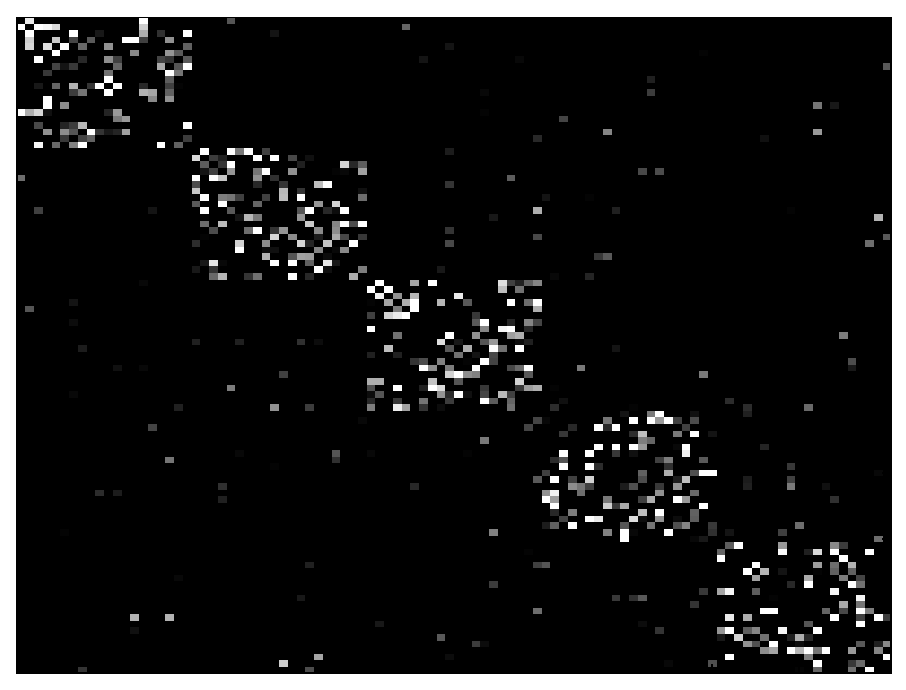
\includegraphics[width=\textwidth]{ViolateSEP}
    \caption{自表示性不满足}
  \end{subfigure}
  \caption{满足和不满足自表示性的邻接矩阵}
  \label{fig:SEP}
\end{figure}

\subsection{自表示的一般性条件}
我们不直接分析 \eqref{eq:multi},    而是引入松弛变量\(E\), 将其转化为有约束的等价形式:
\begin{equation}\label{eq:Opt_original}
  \mathbf{P}_0:\quad \min_{C, E} \;
  \|C^T\|_{2,1}+\frac{\lambda}{2}\|E\|_F^2 \quad
  \text{s.t.} \quad X_\cI=X_{\cI\rightarrow 0}C+E.
\end{equation}
 \eqref{eq:Opt_original} 的对偶问题为:
\begin{equation}\label{eq:Opt_original_dual}
  \mathbf{D}_0:\quad \max_{N} \; \langle N, X_\cI\rangle -
  \frac{1}{2\lambda}\|N\|_F^2 \quad
  \text{s.t.} \quad \|N^T X_{\cI\rightarrow 0}\|_{2,\infty} \leq 1.
\end{equation}
先考虑一个一般的凸优化问题:
\begin{equation}\label{eq:Opt_A_general}
  \quad \min_{C, E} \; \|C^T\|_{2,1}+\frac{\lambda}{2}\|E\|^2_F \quad
  \text{s.t.} \quad B=AC+E.
\end{equation}
我们有\autoref{lemma:OptimalCondition},  它是
\cite{soltanolkotabi2012geometric}中引理~7.1 的拓展.
\begin{lemma}\label{lemma:OptimalCondition}
  给定矩阵\(A\in \R^{d\times n}, B \in \R^{d\times m}\)和指标集\(\cT\subset [n]\),
  若存在矩阵 \(C\in \R^{n\times m},E\in \R^{d\times m}\) 使 \(B=AC+E\)成立, 且
  \(C\) 的行支撑集 \(\cJ\subseteq
  \cT\),同时又存在矩阵\(N\in\R^{d\times m}\)满足
  \begin{align*}
    N^T A_\cJ = \norm(C_{(\cJ)}^T),  & \quad N=\lambda E, \\
    \|N^T A_{\cT\cap \cJ^{c}}\|_{2, \infty} \leq 1, & \quad \|N^T A_{\cT^{c}}\|_{2, \infty}<1,
  \end{align*}
  其中 \(\norm(\cdot)\)是将矩阵的每一非零列归一化为单位向量,
  则 \eqref{eq:Opt_A_general} 的最优解\((C^{*},E^{*})\) 必然有
  \(C^*_{(\cT^c)}=\mathbf{0}\).
\end{lemma}
\begin{proof}
  对最优解 \((C^{*},E^{*})\), 我们有:
  \begin{align}
    \|(C^*)^T\|_{2,1}+\frac{\lambda}{2}\|E^*\|_F^2 =& \|(C^*)^T_{(\cJ)}\|_{2,1}+\|(C^*)^T_{(\cT\cap \cJ^c)}\|_{2,1}+
    \|(C^*)^T_{(\cT^c)}\|_{2,1} + \frac{\lambda}{2} \|E^*\|^2_F\nonumber\\
    \geq&\|C^T_{(\cJ)}\|_{2,1}+\langle \norm(C^T_{(\cJ)}),(C^*)^T_{(\cJ)}-C^T_{(\cJ)}
    \rangle+\|(C^*)^T_{(\cT^c)}\|_{2,1}\nonumber \\
    &+\|(C^*)^T_{(\cT\cap \cJ^c)}\|_{2,1}+\frac{\lambda}{2} \|E\|^2_F +\langle
    \lambda E,E^*-E\rangle\nonumber\\
    =&\|C^T_{(\cJ)}\|_{2,1}+\langle N,A_\cJ(C^*_{(\cJ)}-C_{(\cJ)})\rangle
     +\|(C^*)^T_{(\cT\cap\cJ^c)}\|_{2,1}\nonumber\\
     &+\|(C^*)^T_{(\cT^c)}\|_{2,1} + \frac{\lambda}{2} \|E\|^2_F +\langle
    \lambda E,E^*-E\rangle\nonumber\\
    =&\|C^T_{(\cJ)}\|_{2,1}+\frac{\lambda}{2} \|E\|_F^2+ \|(C^*)^T_{(\cT\cap
    \cJ^c)}\|_{2,1}+\|(C^*)^T_{(\cT^c)}\|_{2,1}\nonumber\\
    &-\langle N,A_{T\cap \cJ^c}C^*_{(\cT\cap \cJ^c)}\rangle
    -\langle N,A_{\cT^c}C^*_{(\cT^c)}\rangle.
    \label{eq:lemma_tmp1}
  \end{align}
  其中 \(\frac{\lambda}{2} \|E^*\|_F^2 \geq \frac{\lambda}{2} \|E\|_F^2 +\langle
  \lambda E,E^*-E\rangle\) 可由Cauchy–Schwarz不等式推得.
  最后一个等式成立是因为 \((C,E)\)和\((C^*,E^*)\)都是可行解, 因此\(\langle
  N,A(C^*-C)\rangle+\langle N,E^*-E\rangle = \langle
  N,AC^*+E^*-(AC+E)\rangle=0\), 同时注意到 \(\| C^T_{(\cJ)}\|_{2, 1} = \|C^T\|_{2, 1}\).

  使用 \(N\) 的不等式条件, 我们有
  \begin{align*}
    \langle N,A_{\cT^c}C^*_{(\cT^c)}\rangle&= \langle A_{\cT^c}^TN,C^*_{(\cT^c)}\rangle
    \leq \|N^T
    A_{T^{c}}\|_{2,\infty}\|(C^*)^T_{(\cT^c)}\|_{2,1}, \\
    \langle N,A_{T\cap \cJ^c}C^*_{(\cT\cap \cJ^c)}\rangle&= 
    \langle A_{T\cap \cJ^c}^TN,C^*_{(\cT\cap \cJ^c)}\rangle
    \leq \|N^T A_{T\cap \cJ^{c}}\|_{2,\infty}\|(C^*)^T_{(\cT\cap
    \cJ^c)}\|_{2,1}. 
  \end{align*}
  将其带入 \eqref{eq:lemma_tmp1},    我们得到:
  \begin{equation*}
    \|(C^*)^T\|_{2,1}+\frac{\lambda}{2} \|E^*\|^2_F \geq \|C^T\|_{2,1}+ \frac{\lambda}{2} 
    \|E\|_F^2 +(1-\|N^T A_{\cT^c}\|_{2, \infty})\|(C^*)^T_{(\cT^c)}\|_{2,1},
  \end{equation*}
  其中 \((1-\|N^T A_{\cT^c}\|_{2, \infty})\) 严格大于 \(0\).

  由于 \((C^*,E^*)\) 是最优解, \(\|(C^*)^T\|_{2,1}+\frac{\lambda}{2}
  \|E^*\|_F^2\leq \|C^T\|_{2, 1}+\frac{\lambda}{2} \|E\|_F^2\). 
  因此 \(\|(C^*)^T_{(\cT^c)}\|_{2,1}=0\) 且 \((C,E)\) 也是最优解.
\end{proof}

因为\(\Omega\)满足 \eqref{eq:nosame},    那么对\(\cI\in \Omega\),
存在\(\cS_\ell\) 满足\( \forall i \in \cI \, y_i \in \cS_\ell\). 
若取 \eqref{eq:Opt_A_general} 中的\(B=X_\cI, A=X_{\cI\rightarrow 0}, \cT=\cI_\ell\),
则如果能构造三元组\((C,E,N)\), 满足\autoref{lemma:OptimalCondition} 的条件,
并且\(C_{(\cI_\ell^c)}=\mathbf{0}\), 那么 \eqref{eq:Opt_original} 的最优解\(C^*\)满足
\(C^*_{(\cI_\ell^c)}=\mathbf{0}\), 再保证\(C^*\)非平凡(不全为零)就可得到自表示性.

\subsection{构造三元组}\label{sec:construct_nu}
为了构造满足条件的三元组,我们希望将表示系数限制在同类点上,于是考虑下面\emph{假想}
\footnote{由于我们不知道每个点的类别,所以实际上无法求解这个问题,因此叫做``假想''}
的优化问题及其对偶问题:
\begin{align}\label{eq:Opt_fictitious2}
  \bP_1: \quad &\min_{C, E} \;
  \|C^T\|_{2,1}+\frac{\lambda}{2}\|E\|_F^2 \quad
  \text{s.t.} \quad X_\cI=X^{(\ell)}_{\cI^c}C+E,\\
  \bD_1: \quad &\max_{N} \; \langle X_\cI, N\rangle -
  \frac{1}{2\lambda} \|N\|_F^2 \quad
  \text{s.t.} \quad \|N^T X^{(\ell)}_{\cI^c}\|_{2, \infty} \leq 1.
  \label{eq:dual_fictitious2}
\end{align}
因为\(\left\{y_i : \forall i \in \cI \right\}\subset \cS_\ell\),
所以\(\bP_1\)相当于只用\(\cS_\ell\)中的数据来表示\(X_\cI\).

 \eqref{eq:Opt_fictitious2} 是有可行解的(我们只需要任取\(C_0\).
算出相应的\(E_0\), \((C_0, E_0)\)即为可行解), 因此由Slater条件\cite{boyd2004convex},
 \eqref{eq:Opt_fictitious2} 和 \eqref{eq:dual_fictitious2} 强对偶,
即 \eqref{eq:Opt_fictitious2} 的最优解\((C, E)\)与 \eqref{eq:dual_fictitious2} 最优解\(N\)满足
\begin{align}\label{eq:strong_dual}
  \|C^T\|_{2,1}+\frac{\lambda}{2}\|E\|_F^2 = \langle X_\cI,N \rangle -
  \frac{1}{2\lambda} \|N\|_F^2   
\end{align}
将\(X_\cI=X^{(\ell)}_{\cI^c}C+E\)代入 \eqref{eq:strong_dual},   稍加整理后得到
\[ \frac{1}{2}\| \sqrt{\lambda}E-\frac{1}{\sqrt{\lambda}}N \|_F^2+
\|C^T\|_{2,1}-\langle C^T, N^T X^{(\ell)}_{\cI^c}\rangle = 0. \]
设\(C\)的行支撑为\(\cJ\), 由\(\|N^T X^{(\ell)}_{\cI^c}\|_{2, \infty} \leq 1\),可得
\begin{align*}
  N=\lambda E, \quad (N^T X^{(\ell)}_{\cI^c})_\cJ =\norm(C_{(\cJ)}^T).
\end{align*}
\(C\in \R^{(n_\ell-m)\times m}\) 对应点\(\{ x_i: i \in \cI_\ell \setminus \cI\}\)
的表示系数, 所以我们将\(C\)按行扩充一些零向量得到\(C^*\)满足
\[ C^*_{\cI_\ell \setminus \cI} = C, \quad C^*_{(i)} = \mathbf{0}
\quad \forall i \in \cI^c_\ell \cup \cI. \]
则\((C^*, E)\)是 \eqref{eq:Opt_original} 的可行解, 同时三元组\((C^*, E, N)\)
满足了\autoref{lemma:OptimalCondition} 的条件, 除了
\begin{equation*}
  \left\|N^T X_{\cI_\ell^c}\right\|_{2,\infty}<1,
\end{equation*}
即我们要给出条件使 \(\forall x \in \mathcal{X}\setminus \mathcal{X}^{(\ell)}\),有
\begin{equation}\label{eq:dual_separation_condition}
   \left \| N^T x\right \|_2 < 1.
\end{equation}
这样根据\autoref{lemma:OptimalCondition} 我们得到的可行解\((C^*, E)\)
就是 \eqref{eq:Opt_original} 的最优解, 再保证\(C^*\)非平凡, 则自表示性成立.

\subsection{对偶矩阵的限制}\label{sec:dual_separation}
我们将 \(N\) 的每一列在子空间 \(\mathcal{S}_{\ell}\) 上投影,得到 \(N_{\parallel}
:=\mathbb{P}_{\cS_\ell}N\), \(N_{\perp} := \P_{\cS_{\ell}^\perp}N\),
其中\(\cS_\ell^\perp\)是\(\cS_\ell\)的正交补空间. 因此
\begin{align}\label{eq:showing_dual_sep_cond}
  \| N^T x \|_2 =& \| N^T (y+z)\|_2 \leq \| N_{\parallel}^T y\|_2+\|
  N_{\perp}^T y\|_2+\|N^T z\|_2 \nonumber\\
  \leq& \mu(\mathcal{X}_{\ell}) \|N_{\parallel}\|_2 + \|N_{\perp}\|_2\|y\|_2
  + \|N_{\parallel}^T \P_{\cS_{\ell}} z\|_2 
  + \|N_\perp^T \P_{\cS_\ell^\perp} z\|_2 .
\end{align}
最后一个不等号是根据\autoref{def:incoherence},   对\(N_\parallel\)做奇异值分解
\(N_\parallel = U\Sigma V^T\), 则
\[
  \|N_\parallel^T y\|_2 = \|V \Sigma U^T y\|_2 = \|\Sigma U^T y\|_2 \le
  \|N_\parallel\|_2 \left\|\P_{\cU_\cI^{(\ell)}} y\right\|_2 \le \mu(\cX_\ell)
  \|N_\parallel\|_2.
\]

\subsubsection{控制 \(\|N_{\parallel}\|_2\)}
我们考察\(N\) 在 \eqref{eq:dual_fictitious2} 中的可行区域:
\[\left\{N \middle| \|N^T X^{(\ell)}_{\cI^c}\|_{2,\infty} \leq 1\right\},\]
等价于
\[\left\{N \middle|\left \| N^T x_i\right\|_2 \leq 1 , \forall \, i \in \cI_\ell
\setminus \cI \right\}.\]
分解可得
\[\| N_{\parallel}^T y_i+N_{\parallel}^T (\mathbb{P}_{\mathcal{S}_{\ell}}z_i)+
N_{\perp}^T z_i\|_2 \leq 1.\]
因为\(y_i \in \cS_\ell\), 所以\(N_\perp^T y_i=\mathbf{0}\). 进而由三角不等式
\begin{equation}\label{eq:relax_constraint}
  \left\| N_{\parallel}^T y_i+N_{\parallel}^T
  (\mathbb{P}_{\mathcal{S}_{\ell}}z_i)\right \|_2
  \leq 1+\|N_{\perp}^T z_i\|_2 \leq 1+\delta\|N_{\perp}\|_2.
\end{equation}

根据多胞体的几何性质,我们有
\begin{align}
  & \| N_{\parallel}^T (y_i+ \mathbb{P}_{\mathcal{S}_{\ell}}z_i) \|_2 \leq
  1+\delta\|N_{\perp}\|_2 \quad \forall i \in \cI_\ell \setminus \cI\nonumber\\
  \Leftrightarrow & \|N_{\parallel}^T x\| \leq 1 \quad \forall x \in \mathcal{P}\left(\frac{Y_{\cI^c}^{(\ell)}+
  \P_{\mathcal{S}_{\ell}}(Z_{\cI^c}^{(\ell)})}{1+\delta\|N_{\perp}\|_2}\right)
  \nonumber\\
  \Rightarrow & \|N_{\parallel}^T x\| \leq 1 \quad \forall x \in \cS_\ell,
  \|x\|_1 \le r\left(\mathcal{P}\left(\frac{Y_{\cI^c}^{(\ell)}+
  \P_{\mathcal{S}_{\ell}}(Z_{\cI^c}^{(\ell)})}{1+\delta\|N_{\perp}\|_2}\right),
  \cS_\ell\right).\label{eq:Geometric_dual}
\end{align}
注意到\(\cP(\cdot)\) 是对称凸包, \(\cP(\cdot)\) 的最大内接球中心在原点.
由于这里都是对子空间\(\cS_\ell\)讨论, 简单起见, 记\(r(\cP, \cS)\)为\(r(\cP)\).
凸包的内接球半径大小能度量点在子空间中分布的均匀程度.
如\autoref{fig:inradius} 所示, 不考虑噪音, 高维空间的三个点\(x_1, x_2,
x_3\)分布在一个二维平面的单位球面上, 当它们分布均匀时, 张出的对称凸包的半径较大, 反之
不均匀时, 半径较小. 内接球半径大说明, 在子空间的各个方向上数据点都有分布,
这样自然能更好地做稀疏表示.

\begin{figure}[tb]
  \centering
  \includegraphics[width=0.8\linewidth]{inradius}
  \caption{数据点分布和其内接球半径的关系}
  \label{fig:inradius}
\end{figure}

我们可以通过子空间\(\cS_\ell\)中无噪音点\(Y^{(\ell)}_{\cI^c}\)的内接球半径控制\(\|N_{\parallel}\|_2\).
\begin{lemma}\label{lemma:circum_inradius}
  对于矩阵 \(A \in \R^{d \times n}\)和子空间\(\cS\subset \R^d\), 
  若\(A\)的每一列\(A_i \in \cS\) 且存在\(r>0\),使得
  \[\|A^Tx\|_2 \leq 1 \quad \forall x \in \cB(0, r)\cap \cS,\]
  其中\(\cB(0, r)\) 表示 \(\R^d\) 中的半径为\(\alpha\)的欧式球,
  那么\(\|A\|_2 \leq \frac{1}{\alpha}\).
\end{lemma}
\begin{proof}
  根据定义我们有
  \begin{align*}
    \|A\|_2 = \max_{x\in \R^n} \frac{\|A^Tx\|_2}{\|x\|_2}
    = \max_{x \in \cS} \frac{\|A^Tx\|_2}{\|x\|_2}
    = \max_{x \in \cB(0,r) \cap \cS} \frac{1}{r} \|A^Tx\|_2
    \leq \frac{1}{\alpha}.
  \end{align*}
\end{proof}

\begin{lemma}\label{lemma:Y_containing_set}
  矩阵 \(Y, Z\in \R^{d \times n}\), 子空间\(\cS \subset \R^d\),
  \(Y\)的每一列在子空间\(\cS\)中,令\(\rho:=\max_{i}\|\P_\cS Z_i\|\),
  那么我们有:
  \begin{equation*}
    r(\cP(Y+\P_\cS Z)) \geq r(\cP(Y)) - \rho
  \end{equation*}
\end{lemma}
\begin{proof}
  令\(X=Y+Z\), 则\(Y+\P_\cS Z=\P_\cS X\). 根据定义\(\cP(\P_\cS X)\) 的边界是集合 \(\mathcal{B}:=
  \left\{y|y=\mathbb{P}_\mathcal{S} X c; \|c\|_1=1\right\}\).
  内接球是凸包内的最大球,因此 \(r(\mathcal{P}(\mathbb{P}_\mathcal{S} X)) =
  \min_{y\in \mathcal{B}} \|y\|\). 对\(y \in \mathcal{B} \) 我们给出下界:
  \begin{align*}
    \|y\| \geq& \|Yc\|-\|\mathbb{P}_\mathcal{S}Z c\|\geq r(\mathcal{P}(Y)) - {\sum}_j{\|\mathbb{P}_\mathcal{S}z_j}\||c_j|
    \geq r(\mathcal{P}(Y)) - \rho\|c\|_1.
  \end{align*}
  因此得证.
\end{proof}

根据 \eqref{eq:Geometric_dual},   \autoref{lemma:circum_inradius} 和\autoref{lemma:Y_containing_set},  
我们可给出\(N_{\parallel}\)的上界:
\begin{align}
  \|N_{\parallel}\|_2 \leq& \frac{1+\delta\|N_{\perp}\|_2}
  {r(\mathcal{P}(Y_{\cI^c}^{(\ell)}+\mathbb{P}_{\mathcal{S}_{\ell}}(Z_{\cI^c}^{(\ell)}))}
  \nonumber \\
  \leq& \frac{1+\delta\|N_{\perp}\|_2}{r{\left( \cQ_{\cI^c}^{(\ell)}\right)}-\delta_1}.\label{eq:nu1_bound}
\end{align}
这个上界依赖于 \(\|N_{\perp}\|_2\), 接下来我们将对其进行分析.

\subsubsection{控制\(\|N_{\perp}\|_2\)}
由于 \(N\) 是 \(\mathbf{D}_1\) 的最优解,由对偶问题的性质,我们有
\[ N=\lambda E=\lambda(X_\cI-X^{(\ell)}_{\cI^c}C). \]
将 \(N\) 投影到 \(\cS^{\perp}_{\ell}\), 我们得到
\(N_{\perp}=\lambda \P_{\cS_{\ell}^{\perp}}(X_\cI-X^{(\ell)}_{\cI^c}C)
= \lambda \mathbb{P}_{\mathcal{S}_{\ell}^{\perp}}(Z_\cI-Z^{(\ell)}_{\cI^c}C)\).
于是对任意\(y\in \R^d, \|y\|_2=1\) 有
\begin{align}
  \|N_{\perp}^T y\|_2 & \leq\lambda \left(\|\mathbb{P}_{\mathcal{S}_{\ell}^{\perp}}Z_\cI\|_2
  +\|C^T (\mathbb{P}_{\mathcal{S}_{\ell}^{\perp}}Z^{(\ell)}_{\cI^c})^T y\|_2\right)\nonumber\\
  & \leq \lambda\left( \sqrt{m} \delta + \|C^T \ty\|_2\right) \nonumber\\
  & \leq \lambda\left( \sqrt{m} \delta + \sum_j |\ty_j|\|C_{(j)}\|_2\right) \nonumber\\
  & \leq \lambda\left( \sqrt{m} \delta + \|\ty\|_{\infty}\|C^T\|_{2,1}\right) \nonumber\\
  & \leq \lambda \delta(\Cgl+\sqrt{m}) \leq \lambda\delta\sqrt{m}(\Cgl+1).
  \label{eq:bounding_nu2_0}
\end{align}
其中\(\ty=(\mathbb{P}_{\mathcal{S}_{\ell}^{\perp}}Z^{(\ell)}_{\cI^c})^Ty\),
而\(\|\ty\|_\infty \leq \|z_i\|_2 \|y\|_2 \leq
\delta\). 由 \eqref{eq:bounding_nu2_0} 得
\begin{align}
  \|N_{\perp}\|_2 = \max_{\|y\|_2=1} \|N^T y\|_2 \le \lambda\delta\sqrt{m}(\Cgl+1).
  \label{eq:bounding_nu2}
\end{align}

下面我们给出 \(\Cgl\)的上界.
因为 \((C,E)\) 是 \eqref{eq:Opt_fictitious2} 的最优解,所以对任何可行解 \((\tC ,\tE)\)
都有 \(\Cgl+\frac{\lambda}{2}\|E\|^2_F \leq \tCgl+\frac{\lambda}{2}\|\tilde{E}\|_F^2\).
令 \(\tC\) 为下面无噪音优化问题的解
\begin{align}\label{eq:Opt_y only}
\min_{c} \; \Cgl \quad
\text{s.t.} \quad Y_\cI=Y^{(\ell)}_{\cI^c}C,
\end{align}
由强对偶性,
\[\tCgl = \max_{N}\left\{\langle N,Y_\cI\rangle | \|N^T
Y^{(\ell)}_{\cI^c}\|_{2, \infty}\leq 1\right\}.\]
根据\autoref{lemma:circum_inradius},   对偶问题的最优解 \(\tilde{N}\) 满足
\(\|\tilde{N}\|_2 \leq \frac{1}{r(\mathcal{Q}_{\cI^c}^{(\ell)})}\).于是
\[\tCgl = \langle\tilde{N},Y_\cI\rangle \leq
\frac{m}{r(\mathcal{Q}_{\cI^c}^{(\ell)})}.\]

同时 \(\tilde{E} = Z_\cI - Z_{\cI^c}^{(\ell)}\tC\), 所以 
\[\|\tilde{E}\|_F^2 \leq (\|Z_\cI\|_F+\sum_{j,k} \|z_j\||\tC_{j,k}|)^2
\leq \delta^2 (\sqrt{m} + \|\tC\|_1)^2\leq m \delta^2(1+ \tCgl)^2,\]
于是
\begin{align}
  \Cgl \leq& \tCgl +
  \frac{\lambda}{2}\|\tilde{E}\|_F^2-\frac{\lambda}{2}\|E\|_F^2\nonumber \\
  \leq& \frac{m}{r{(\mathcal{Q}_{\cI^c}^{(\ell)})}}+\frac{\lambda}{2}m\delta^2
  \left[1+\frac{m}{r{(\mathcal{Q}_{\cI^c}^{(\ell)})}}\right]^2-\frac{1}{2\lambda}\|N_{\perp}\|_2^2,
  \label{eq:c_bound}
\end{align}
注意到 \(\frac{\lambda}{2}\|E\|_F^2=\frac{1}{2\lambda}\|N\|_F^2
\geq\frac{1}{2\lambda}\|N_{\perp}\|_F^2 \geq\frac{1}{2\lambda}\|N_{\perp}\|_2^2\).
将 \eqref{eq:c_bound} 带入 \eqref{eq:bounding_nu2} 得
\[\|N_{\perp}\|_2 \leq \lambda \delta \sqrt{m} 
\left(\frac{m}{r(\mathcal{Q}_{\cI^c}^{(\ell)})}+\frac{\lambda}{2}\delta^2m
\left[1+\frac{m}{r(\mathcal{Q}_{\cI^c}^{(\ell)})}\right]^2+1\right)
-\frac{\delta}{2}\sqrt{m}\|N_{\perp}\|_2^2 \]
对上式稍加整理得到
\[\|N_{\perp}\|_2+\frac{\delta}{2}\sqrt{m}\|N_{\perp}\|_2^2\leq
  \lambda\delta\sqrt{m}\left(\frac{m}{r(\mathcal{Q}_{\cI^c}^{(\ell)})}+1\right)+
  \frac{\delta}{2}\sqrt{m} \left[\lambda\delta\sqrt{m}
  \left(\frac{m}{r(\mathcal{Q}_{\cI^c}^{(\ell)})}+1\right)\right]^2,\]
由于函数 \(f(\alpha)=\alpha+\frac{\delta}{2}\sqrt{m}\alpha^2\) 在 \(\alpha>0\)
时单调递增,则上面的不等式可以推出
\begin{equation}\label{eq:nu2_bound}
  \|N_{\perp}\|_2 \leq \lambda\delta\sqrt{m}\left(\frac{m}{r(\mathcal{Q}_{\cI^c}^{(\ell)})}+1\right),
\end{equation}
即我们需要的 \(\|N_{\perp}\|_2\) 的上界.

\subsubsection{ \(\|N^T x\|_2<1\) 所需的条件}
结合 \eqref{eq:showing_dual_sep_cond},  \eqref{eq:nu1_bound} 和 \eqref{eq:nu2_bound},    
我们可以得出 \(\|N^T x\|_2\) 的上界:
\begin{align*}
  \|N^T x\|_2 \leq& (\mu(\mathcal{X}_{\ell})+\|\mathbb{P}_{\mathcal{S}_{\ell}}z\|) 
  \|N_{\parallel}\|_2+(\|y\|+\|\mathbb{P}_{\mathcal{S}_{\ell}^{\perp}}z\|)\|N_{\perp}\|_2\\
  \leq&\frac{\mu(\cX_\ell)+\delta_1}{r{\left(\cQ_{\cI^c}^{(\ell)}\right)}-\delta_1}
  +\left(\frac{(\mu(\mathcal{X}_{\ell})+\delta_1)\delta}{r{\left( \mathcal{Q}_{\cI^c}^{(\ell)}\right)}-\delta_1}+1+\delta\right)
  \|N_{\perp}\|_2\\
  \leq& \frac{\mu(\mathcal{X}_{\ell})+\delta_1}{r{\left( \mathcal{Q}_{\cI^c}^{(\ell)}\right)}-\delta_1} +
  \lambda\delta(1+\delta)\sqrt{m}
  \left(\frac{m}{r(\mathcal{Q}_{\cI^c}^{(\ell)})}+1\right) \\
  &+ \frac{\lambda\delta^2\sqrt{m}(\mu(\mathcal{X}_{\ell})+\delta_1)}
  {r{\left( \mathcal{Q}_{\cI^c}^{(\ell)}\right)}-\delta_1}\left(\frac{m}{r(\mathcal{Q}_{\cI^c}^{(\ell)})}+1\right).
\end{align*}
简单起见,我们把第二个 \(r(\mathcal{Q}_{\cI^c}^{(\ell)})\) 松弛成 \(r(\mathcal{Q}_{\cI^c}^{(\ell)})-\delta_1\).
这样对偶分离条件就被下式保证
\begin{multline}\label{eq:dual_cond_full}
   \lambda\sqrt{m}\delta(1+\delta)
  +\frac{\lambda\delta^2 m^{3/2}(\mu(\mathcal{X}_{\ell})+\delta_1)}
  {r{\left( \mathcal{Q}_{\cI^c}^{(\ell)}\right)}(r{\left(
    \mathcal{Q}_{\cI^c}^{(\ell)}\right)}-\delta_1)} \\
  +\frac{\mu(\mathcal{X}_{\ell})+\delta_1 +\lambda m^{3/2}\delta(1+\delta)+
  \lambda\sqrt{m}\delta^2(\mu(\mathcal{X}_{\ell})+\delta_1)}
  {r{\left( \mathcal{Q}_{\cI^c}^{(\ell)}\right)}-\delta_1}<1.
\end{multline}
记 \(\rho:=\lambda\sqrt{m}\delta\), 假设\(\delta<r{\left(\cQ_{\cI^c}^{(\ell)}\right)}\)
和\((\mu(\mathcal{X}_{\ell})+\delta_1)<1\), 那么我们有下面的不等式
\begin{align*}
  \frac{\lambda\sqrt{m}\delta^2(\mu(\mathcal{X}_{\ell})+\delta_1)}
  {r{\left( \mathcal{Q}_{\cI^c}^{(\ell)}\right)}-\delta_1}
  +\frac{\lambda\delta^2 m^{3/2}(\mu(\mathcal{X}_{\ell})+\delta_1)}
  {r{\left( \mathcal{Q}_{\cI^c}^{(\ell)}\right)}(r{\left( \mathcal{Q}_{\cI^c}^{(\ell)}\right)}-\delta_1)}
  < \frac{\rho (m+\delta)}{r{\left( \mathcal{Q}_{\cI^c}^{(\ell)}\right)}-\delta_1}.
\end{align*}
用上式化简 \eqref{eq:dual_cond_full} 左边, 可得一个充分条件
\begin{equation}\label{eq:dual_cond_simp}
  \mu(\mathcal{X}_{\ell}) +\rho [2m+(1+m)\delta] +\delta_1
  < \left(1-\rho(1+\delta)\right)(r(\mathcal{Q}_{\cI^c}^{(\ell)})-\delta_1).
\end{equation}
把 \eqref{eq:dual_cond_simp} 一般化到所有子空间的所有分组上,
则必须对每个\(\ell = 1,...,L\) 成立:
\begin{equation}\label{eq:Thm1_all}
  \mu(\mathcal{X}_{\ell}) +\rho [2m+(1+m)\delta] +\delta_1
  < \left(1-\rho(1+\delta)\right)\left(\min_{\{\cI: \cI\in \Omega_\ell\}}r(\mathcal{Q}^{(\ell)}_{\cI^c})-\delta_1\right).
\end{equation}

\subsection{避免平凡解}\label{sec:avoid_trivial}
除了满足自表示以外, 我们还要要求解是非平凡的. 不难看出,只要当 \(\lambda\)
足够大时, 平凡解 \((\mathbf{0}, X_\cI)\) 肯定不是最优解.

\begin{lemma}\label{lemma:avoid_trivial}
  对于 \eqref{eq:Opt_A_general},   当 \(\lambda > \frac{1}{\max_{i,j} |A_i^T
B_j|}\) 时,其最优解一定是非平凡的.
\end{lemma}
\begin{proof}
  我们只要说明存在一个非平凡解比平凡解更优即可. 设 \(i, j\) 为 \(|A_i^T
  B_j|\) 取到最大时的下标, 构造可行解\(C\), 
  取\(C_{i,j} = \frac{\lambda |A_i^T B_j|-1}{\lambda \|A_i\|_2^2} \sign(A_i^T B_j)\) 
  其余为\(0\), 则\(C\) 非平凡.我们有
  \begin{align*}
    \frac{\lambda}{2} \|B_j - A_i C_{i, j} \|_2^2 + |C_{i, j}| =& \frac{\lambda}{2}
    \|B_j\|_2^2 + \frac{\lambda}{2} \|A_i\|_2^2 C_{i,j}^2 +\left( 1-\lambda |A_i^T B_j|
    \right)C_{i,j} \\
    =&\frac{\lambda}{2} \|B_j\|_2^2 - \frac{(\lambda|A_i^T B_j| -1)^2}
    {2 \lambda \|A_i\|_2^2 }\\
    <& \frac{\lambda}{2} \|B_j\|_2^2. 
  \end{align*}
  因此最优解一定非平凡.
\end{proof}

我们要求 \eqref{eq:Opt_fictitious2} 的解非平凡, 因此需要考虑
\(\|[X_{\cI^c}^{(\ell)}]^T X_\cI \|_{\infty} \).
设\(i, i_0\in \cI_\ell \setminus \cI, \, j, j_0\in
\cI\), 且
\begin{gather*}
x_{i_0}^T x_{j_0}=\left\|\left[X_{\cI^c}^{(\ell)}\right]^T X_\cI\right\|_\infty, \\
y_i^T y_j=\left\|\left[ Y_{\cI^c}^{(\ell)}\right]^T Y_\cI\right\|_\infty ,
\end{gather*}
则
\begin{align}
  \left\|[X_{\cI^c}^{(\ell)}]^TX_\cI\right\|_{\infty}&=\left|\langle x_{i_0},
  x_{j_0}\rangle\right|  \geq \left|\langle x_i, x_j\rangle\right|\nonumber\\
  &= \left|\langle y_i, y_j\rangle  + \langle y_i, z_j\rangle + \langle z_i, y_j\rangle + \langle z_i, z_j\rangle\right|\nonumber\\
  &\geq \left|\langle y_i, y_j\rangle\right| - \left|\langle y_i, z_j\rangle + \langle z_i, y_j\rangle + \langle z_i, z_j\rangle\right|\nonumber\\
  & = \left\|[y_{\cI^c}^{(\ell)}]^Ty_i\right\|_{\infty} - \left|\langle y_i, z_j\rangle + \langle z_i, y_j\rangle + \langle z_i, z_j\rangle\right|\nonumber\\
  &\geq r(\mathcal{Q}^{(\ell)}_{\cI^c}) - 2\delta - \delta^2. \label{eq:lowerbounding_maX_affinity}
\end{align}
最后一个不等式成立是因为 \(\mathcal{Q}^{(\ell)}_{\cI^c}\) 
的内接球半径是集合 \(\{\| [ Y_{\cI^c}^{(\ell)}]^T w\|_\infty: w
\in  \mathcal{S}_{\ell}\} \) 的下界. 因此只要
\begin{equation}\label{eq:lambda_low}
  \lambda > \frac{1}{ r(\mathcal{Q}^{(\ell)}_{\cI^c}) - 2\delta - \delta^2},
\end{equation}
 \eqref{eq:Opt_fictitious2} 的解就是非平凡的.

\subsection{自表示定理}
将上面几小节的内容总结一下可以得到MT-SSC的自表示定理
\begin{theorem}\label{thm:mt_SEP}
  在带噪音的确定性模型下, 若给定指标集族\(\Omega\), 满足 \eqref{eq:nointer} 
 \eqref{eq:full} 和 \eqref{eq:nosame},  且\(|\cI|=m, \, \forall\, \cI \in \Omega\). 对任意\(\ell \in [L]\),
  若\(\mu(\cX_\ell)<1-\delta_1\), \(\min_{\cI\in
  \Omega_\ell} r\left(\cQ^\ell_{\cI^c}\right) > \delta\), 同时能取出
  参数\(\lambda > \frac{1}{ r(\mathcal{Q}^{(\ell)}_{\cI^c}) - 2\delta -\delta^2}\),
  使得
  \[\mu(\cX_\ell) +\sqrt{m}\delta\lambda \left[2m+(1+m)\delta \right] +\delta_1
  < \left(1-\sqrt{m}\delta\lambda(1+\delta)\right)\left(\min_{\cI\in \Omega_\ell}
  r(\cQ^{(\ell)}_{\cI^c})-\delta_1\right)\]
  成立. 那么MT-SSC得到的解具有自表示性.
\end{theorem}
需要指出的是虽然在\autoref{thm:mt_SEP} 中\(m\)越大条件越不容易满足,
但是这并不代表MT-SSC表现一定比SSC差. 只是MT-SSC相对SSC不等式放缩更难处理,
所以得到的理论条件较苛刻.
